\documentclass{beamer}
\usetheme{Berlin}
\usecolortheme{dolphin}
\usepackage{color, graphicx}

\title{An Introduction to Bayesian Methods for Survival Analysis}
\author{Sarah Lotspeich, Elizabeth Sigworth}
\institute{Vanderbilt University}
\date{5 December 2017}

\begin{document}

\begin{frame}
\titlepage
\end{frame}

\begin{frame}
\frametitle{Outline}
\tableofcontents
\end{frame}

\begin{frame}[c]
\begin{center}
\Huge
``Be Bayesian or go home.''  
\huge
-Dr. Frank Harrell, 2017
\end{center}
\end{frame}

\section{The Bayesian Paradigm}
\begin{frame}
\frametitle{A Refresher on Posterior Distributions}
Specify a probability model for the observed data given a vector of unknown parameters $\pmb{\theta}$, leading to a likelihood function $L(\pmb{\theta}|\text{data})$. Assume $\pmb{\theta}$ is random and has \underline{prior distribution} $\pi(\pmb{\theta})$. Inference concerning $\pmb{\theta}$ based on prior distribution is obtained from Bayes' Theorem. 
$$\pi(\pmb{\theta}|\text{data}) = \frac{L(\pmb{\theta}|\text{data})\pi(\pmb{\theta})}{\int_{\Theta}L(\pmb{\theta}|\text{data})\pi(\pmb{\theta}) d\pmb{\theta}}$$
where $\Theta$ denotes the parameter space of $\pmb{\theta}$. \footnotemark
\begin{itemize}
\item Note: the denominator here is the \underline{marginal distribution} of the data, which often does not have a closed form. 
\item Without this, it is challenging to analytically solve for $\pi(\pmb{\theta}|\text{data})$. 
\end{itemize}
\footnotetext[1]{Ibrahim, et al. (2001)}
\end{frame}

\begin{frame}
\frametitle{Connecting the Prior and Posterior}
We can see that $\pi(\pmb{\theta}|\text{data})$ is proportional to the likelihood $L(\pmb{\theta}|\text{data})$ multiplied by the prior $\pi(\pmb{\theta})$
$$\pi(\pmb{\theta}|\text{data}) \propto L(\pmb{\theta}|\text{data})\pi(\pmb{\theta})$$
\begin{itemize}
\item Contributions from the data and the prior through the likelihood and prior distributions, respectively. 
\end{itemize}
\end{frame}

\begin{frame}
\frametitle{Why Bayes?}
\begin{itemize}
\item Historical data formally incorporated into current analysis through \color{orange} power prior\color{black}.
\item Model comparisons via \color{orange} Bayes Factors\color{black}.
$$BF_{\text{model A}, \text{model B}} = \frac{P(\text{data}|\text{model A})}{P(\text{data}|\text{model B})}$$ 
\item \color{orange}Missing values \color{black}treated as parameters. 
\item MCMC sampling techniques allow us to make exact inference for \color{orange}any sample size \color{black}without relying on asymptotic approximations. 
\end{itemize}
\end{frame}

\section{MCMC Posterior Sampling}
\begin{frame}
\frametitle{The Problem with Marginal Distributions}
Methods to sample from the posterior distribution without knowing the marginal include Gibbs sampler and other Markov chain Monte Carlo sampling algorithms. 
\begin{itemize}
\item The idea in Gibbs sampling is to generate posterior samples by sweeping through each variable (or block of variables) to sample from its conditional distribution with the remaining variables fixed to their current values.\footnotemark
\end{itemize}
\footnotetext[2]{Yildirim (2012)}
\end{frame}

\begin{frame}
\frametitle{Gibbs sampler}
We have $\pmb{\theta} = (\theta_1, \theta_2, \ldots, \theta_p)'$ be a $p$-dimensional vector of parameters, and $\pi(\pmb{\theta}|\text{data})$ is the posterior given data. 
\begin{enumerate}
\item[Step 0.] Choose an arbitrary starting point $\pmb{\theta}_{0} = (\theta_{1,0}, \theta_{2,0}, \ldots, \theta_{p,0})'$, and set $i = 0$.
\item [Step 1.] Generate $\pmb{\theta}_{i+1} = (\theta_{1,i+1}, \theta_{2,i+1}, \ldots, \theta_{p,i+1})'$ as follows:
	\begin{itemize}
	\item Generate $\pmb{\theta}_{1,i+1} \sim \pi(\theta_1|\theta_{2,i}, \ldots, \theta{p,i},\text{data})$
	\item Generate $\pmb{\theta}_{2,i+1} \sim \pi(\theta_2|\theta_{1,i+1}, \theta_{3,i}, \ldots, \theta{p,i},\text{data})$
	\item $\vdots$
	\item Generate $\pmb{\theta}_{p,i+1} \sim \pi(\theta_p|\theta_{1,i+1}, \theta_{2,i+1}, \ldots, \theta_{p-1,i+1}, \text{data})$
	\end{itemize}
\item [Step 2.] Set $i = i+1$, and go to Step 1.
Stop when $\pmb{\theta} = (\theta_1, \theta_2, \ldots, \theta_p)'$ converges.\footnotemark[1]
\end{enumerate}
\footnotetext[1]{Ibrahim, et al. (2001)}
\end{frame}

\begin{frame}
\frametitle{Gibbs Sampler Example: Setup}
Consider 20 subjects in an observational study. Denote the number dead due to natural causes as random variable $D \sim Bin(20,\theta)$.  Suppose a previous study found that, on average, $40\%$ of people die due to natural causes. Based on this, we impose a beta prior on $\theta$, i.e. $\theta \sim Beta(a,b)$. We choose parameters $a$ and $b$ such that 
\begin{center}
$E(\theta) = \frac{a}{a+b} = 0.40$
\end{center}
This gives us $a = 4$ and $b = 6$. We want to be able to sample from the posterior distribution for $\theta|\text{data}$. 
\end{frame}

\begin{frame}
\frametitle{Gibbs Sampler Example: Posterior Distribution}
For a beta-binomial model, we have the following conjugate posterior
\begin{eqnarray*}
\pi(\theta|D) &=& \frac{f(d;\theta)\pi(\theta)}{f(d)} \\
&=& \frac{{20 \choose d}\theta^{d}(1-\theta)^{20-d} \frac{\Gamma(4 + 6)}{\Gamma(4)\Gamma(6)}\theta^{4-1}(1-\theta)^{6-1}}{{20 \choose d} \frac{\Gamma(4 + 6)}{\Gamma(4)\Gamma(6)} \frac{\Gamma(4 + d)\Gamma(6 + 20 - d)}{\Gamma(4+6+20)}} \\
&=& \frac{\Gamma(4+6+20)}{\Gamma(4 + d)\Gamma(6 + 20 - d)}\theta^{4+d-1}(1-\theta)^{26-d} 
\end{eqnarray*}
Which we recognize as posterior distribution $\theta|D \sim Beta(4+d, 26-d)$. 
\end{frame}

\begin{frame}[fragile]
\frametitle{Gibbs Sampler Example: R Code\footnotemark}
\begin{verbatim}
n <- 20; a <- 4; b <- 6 #setup parameters

it <- 1500 #number of iterations
d= rep(NA,it); theta=rep(NA,it) 
d[1]=1; theta[1]=0.5 # set arbitrary initial values

# Perform Gibbs iterations
for (i in 2:it)
{
  d[i] =rbinom(1,size=n,prob=th[i-1])
  theta[i] = rbeta(1,a+d[i],b+n-d[i])
}
\end{verbatim}
\footnotetext[3]{Huerta (2012)}
\end{frame}

\begin{frame}
\begin{center}
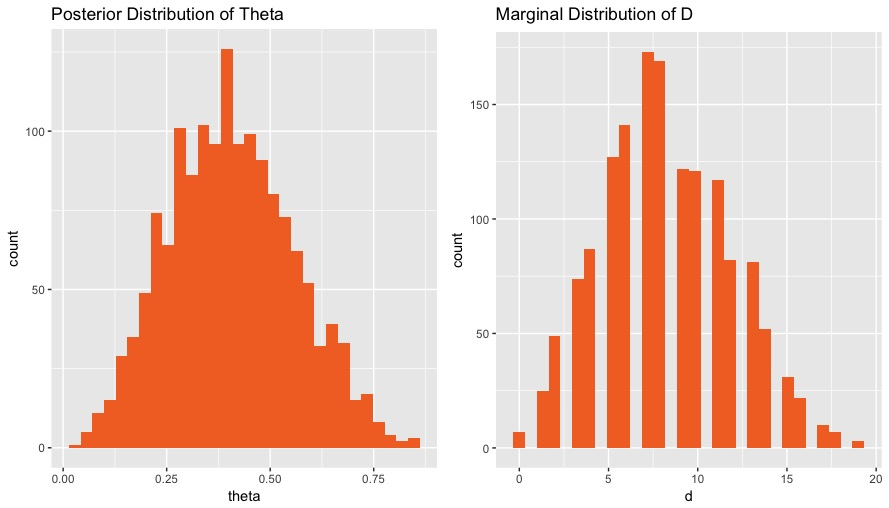
\includegraphics[scale=0.35]{Rplot.jpeg}
\end{center}
\end{frame}

\section{Power Priors}
\begin{frame}
\frametitle{We've Got the Power [Prior]}
The \underline{power prior} is defined to be the likelihood function based on historical data raised to a power $a_{0}$ where $0 \leq a_0 \leq 1$. 
\begin{itemize}
\item Scalar parameter $a_0$ controls the influence of the historical data on the current data.  
\end{itemize}
The power prior distribution of $\pmb{\theta}$ is 
\begin{center}
$\pi(\pmb{\theta}|\text{data}_0, a_0) \propto L(\pmb{\theta}|\text{data}_0)^{a_0}\pi_0(\pmb{\theta}|c_{0})$
\end{center}
\begin{itemize}
\item $\text{data}_0$: historical data from a similar previous study 
\item $a_0:$ relative precision parameter for historical data $\text{data}_0$
\item $c_0$: a specified hyperparameter for the initial prior that controls the impact of $\pi_0(\pmb{\theta}|c_{0})$ on the entire prior $\pi(\pmb{\theta}|\text{data})$
\end{itemize}
\end{frame}

\begin{frame}
\frametitle{Controlling the Influence of Past Data}
\begin{itemize}
\item When \color{orange}$a_0 = 1$\color{black}, the power prior distribution corresponds to the posterior distribution of $\pmb{\theta}$ from the historical study (no change for current study).
\item When \color{orange}$a_0 = 0$\color{black}, the power prior distribution does not depend on the historical data at all (i.e. no incorporation of historical data for current study). 
\item Thus, $a_0$ allows the investigator to select the influence of historical data on the current study. 
	\begin{itemize}
	\item Want $a_0$ closer to 1 when the studies are very similar. 
	\item Want $a_0$ closer to 0 when sample sizes are different or there is heterogeneity between studies. 
	\end{itemize} 
\end{itemize}
\end{frame}

\begin{frame}
\frametitle{Hierarchical Power Prior Specification}
Incorporate a prior for $a_0$, $\pi(a_0|\pmb{\gamma}_0)$, into the prior for $\pmb{\theta}|\text{data}_0, a_0$ to get
\begin{center}
$\pi(\pmb{\theta}, a_0|\text{data}_0) \propto L(\pmb{\theta}|\text{data}_0)^{a_0}\pi_0(\pmb{\theta}|c_{0})\pi(a_0|\pmb{\gamma}_0)$
\end{center}
where $\pmb{\gamma}_0$ is a specified vector of hyperparameters. A natural choice for $\pi(a_0|\pmb{\gamma}_0)$ is a \color{orange} beta prior\color{black}. 
\end{frame}

\section{Bayesian Parametric Models}
\begin{frame}
\frametitle{Exponential Model}
Consider event times $X_i \overset{iid}{\sim} Expo(\lambda)$ for $i = 1, \ldots, n$. 

Define:
\begin{itemize}
\item$X_i$: time on study for observation $i$
\item $\delta_i$: event indicator for observation $i$ ($=0$ if right censored, $=1$ if event observed)
\item $T_i:$ time to event for observation $i$ (if $\delta_i = 1$, $X_i = T_i$)
\item $C_i:$ time to right censoring for observation $i$ (if $\delta_i = 0$, $X_i = C_i$)
\end{itemize}
\end{frame}

\begin{frame}
\frametitle{Exponential Model: Likelihood}
\begin{eqnarray*}
L(\lambda|\text{data}) &=& \prod_{i=1}^{n} f(x_i|\lambda)^{\delta_i}S(x_i|\lambda)^{1-\delta_i} \\
&=& \prod_{i=1}^{n} (\lambda \exp\{-\lambda x_i\})^{\delta_i}(\exp\{-\lambda x_i\})^{1-\delta_i} \\
&=& (\lambda \exp\{-\lambda x_i\})^{\sum_{i=1}^{n}\delta_i}(\exp\{-\lambda x_i\})^{n-\sum_{i=1}^{n}\delta_i} \\
&=& (\lambda^{\sum_{i=1}^{n}\delta_i} \exp\{-\sum_{i=1}^{n}\delta_i\lambda x_i\})(\exp\{-(n-\sum_{i=1}^{n}\delta_i)\lambda x_i\}) \\
&=& \lambda^{d}\exp\{-\lambda \sum_{i=1}^{n}x_i\} \text{ where we let }d = \sum_{i=1}^{n}\delta_i
\end{eqnarray*}
\end{frame}

\begin{frame}
\frametitle{Exponential Model: Prior Distribution}
For exponential event times, the conjugate prior is the gamma distribution: $\lambda \sim Gamma(\alpha_0, \lambda_0)$ with density
$$\pi(\lambda|\alpha_0,\lambda_0) \propto \lambda^{\alpha_0-1}exp\{-\lambda_0 \cdot \lambda\}.$$
\end{frame}

\begin{frame}
\frametitle{Exponential Model: Posterior Distribution}
Based on this prior, we have posterior distribution for $\lambda$
\begin{eqnarray*}
\pi(\lambda|\text{data}) &\propto& L(\lambda|\text{data}) \pi(\lambda|\alpha_0,\lambda_0) \\
&\propto& \left(\lambda^{\sum_{i=1}^n \delta_i} \exp\left\{-\lambda \sum_{i=1}^n x_i \right\} \right) \left(\lambda^{\alpha_0-1}\exp(-\lambda_0\lambda) \right) \\
&\propto& \lambda^{\alpha_0+d - 1}\exp\left\{-\lambda(\lambda_0 + \sum_{i=1}^n x_i ) \right\}
\end{eqnarray*}
We recognize this as a \color{orange}$Gamma(\alpha_0 + d, \lambda_0 + \sum_{i=1}^{n}x_i)$ \color{black}distribution. 
\end{frame}

\begin{frame}
\frametitle{Exponential Model: Posterior Mean and Variance}
Based on the posterior distribution $\lambda|\text{data} \sim Gamma(\alpha_0 + d, \lambda_0 + \sum_{i=1}^{n}x_i)$ we have the following estimates for the mean and variance of the parameter $\lambda$ in $X_i \sim Expo(\lambda)$.
\begin{itemize}
\item $\text{E}(\lambda|\text{data}) = \frac{\alpha_0 + d}{\lambda_0 + \sum_{i=1}^n x_i}$
\item $\text{Var}(\lambda|\text{data}) = \frac{\alpha_0 + d}{(\lambda_0 + \sum_{i=1}^n x_i)^2}$
\end{itemize} 
\end{frame}

\section{Questions}
\begin{frame}[c]
\begin{center}
\Huge
Questions? 
\end{center}
\end{frame}

\section{References}
\begin{frame}
\frametitle{References}
\begin{enumerate}
\item[1] Ibrahim, Joseph George, et al. Bayesian Survival Analysis. Springer, 2010.
\item[2] Yildirim, Ilker. Bayesian Inference: Gibbs Sampling. 2012, Bayesian Inference: Gibbs Sampling.
\item[3] Huerta, Gabriel. Some Examples on Gibbs Sampling and Metropolis-Hastings methods. 2012, Some Examples on Gibbs Sampling and Metropolis-Hastings methods. 
\end{enumerate}
\end{frame}

\end{document}